\scanpage{23}
\margin{n\textsuperscript{o}329}
\uline{CHAPITRE II}

\figure{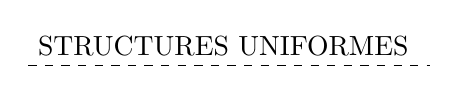
\begin{tikzpicture}\node[anchor=south west] at (0,0) {STRUCTURES UNIFORMES};\draw[dashed] (0,0)--(5.1,0);\end{tikzpicture}}

1. Espaces uniformes.

\uline{1. Définition d'une structures uniforme.}

DEFINITION 1. \uline{Etant donné un ensemble} $X$, \uline{on dit qu'un ensemble} $\underline U$ \uline{de parties de}
$X\times X$ \uline{définit sur} $X$ \uline{une structure uniforme s'il satisfait aux axiomes}
$(F_{\mathrm I})$ \uline{et} $(F_{\mathrm{II}})$ \uline{du chap.} I, 3\textsuperscript{e} éd., § 6, n\textsuperscript{o}1, \uline{et aux axiomes suivants} :

$(U_{\mathrm I})$\quad \uline{Tout ensemble de} $\underline U$ \uline{contient la diagonale} $\Delta$ (fig.2).

$(U_{\mathrm{II}})$\quad \uline{La relation} $V\in\underline U$ \uline{entraîne} $V^{-1}\in\underline U$.

$(U_{\mathrm{III}})$\quad \uline{Quel que soit} $V\in\underline U$, \uline{il existe} $W\in\underline U$ \uline{tel que} $W\circ W\in V$.

\uline{On dit que les ensembles de} $\underline U$ \uline{sont les entourages de la structures uniforme définie sur} $X$ \uline{par} $\underline U$.

Si $V$ est un entourage d'une structure uniforme sur $X$, on conviendra de
considérer la phrase ``x et y sont voisins d'ordre V'' comme une relation équivalente à $(x,y)\in V$.

\uline{Remarques.}-- 1) Pour rendre le langage plus imagé, on pourra employer
les expressions ``x et y sont assez voisins'' et ``x et y sont aussi
voisins qu'on veut'' dans certains énoncés. Par exemple, on dira
qu'une relation $R\{x,y\}$ est vérifiée \uline{si x et y sont assez voisins},
lorsqu'il existe un entourage $V$ tel que la relation $(x,y)\in V$ \uline{entraîne} $R\{x,y\}$.

2) La conjonction des axiomes $(U_{\mathrm{II}})$ et $(U_{\mathrm{III}})$ est (compte tenu des autres axiomes des structures uniformes) équivalente à l'axiome.

$(U_a)$\quad \uline{Quel que soit} $V\in\underline U$, \uline{il existe} $W\in\underline U$ \uline{tel que} $W\unsure{\circ}W^{-1}\in V$.

Il est clair en effet que $(U_{\mathrm{II}})$ et $(U_{\mathrm{III}})$ entraînent $(U_a)$. Inversement, si $(U_a)$ est vérifié, on a $W^{-1}=\Delta\circ W^{-1}\subset V$ d'après $(U_{\mathrm I})$ ;
\mspage{22}
